\documentclass[11pt,a4paper]{article}

\usepackage[T1]{fontenc}
\usepackage[utf8]{inputenc}
\usepackage{lmodern}
\usepackage[a4paper,margin=1in]{geometry}
\usepackage{graphicx}
\usepackage{booktabs}
\usepackage{longtable}
\usepackage{tabularx}
\usepackage{array}
\usepackage{enumitem}
\usepackage[hidelinks]{hyperref}

\setlength{\parskip}{0.5em}
\setlength{\parindent}{0pt}
\renewcommand{\arraystretch}{1.2}

\title{Safe Project Architecture}
\author{Project documentation companion}
\date{\today}

\begin{document}

\maketitle
\tableofcontents
\newpage

\section{Project Application}

This project implements the firmware for a prototype electronic safe controller built on an
STM32 NUCLEO-L476RG platform. The application combines authentication, lockout protection,
operator feedback, and a small administrator console in a single embedded control loop.

The current prototype demonstrates these capabilities:

\begin{itemize}[leftmargin=1.5em]
\item user PIN entry through a 4x4 matrix keypad
\item operator and user feedback on a 4-digit seven-segment display
\item LED and buzzer indication for armed, admin, success, error, and lockout conditions
\item configurable timed lockout after repeated failed attempts
\item administrative functions for PIN change, lockout configuration, sound control, and diagnostics
\end{itemize}

At the application level, the system behaves like the front panel of an electronic safe:

\begin{itemize}[leftmargin=1.5em]
\item normal users enter a 4-digit PIN
\item administrators enter a 6-digit PIN to reach a maintenance menu
\item the display and indicators continuously reflect the current security state
\item the firmware enforces a lockout after too many failed attempts
\end{itemize}

\section{Hardware Platform}

The hardware is organized around three visible elements:

\begin{itemize}[leftmargin=1.5em]
\item an STM32 NUCLEO-L476RG development board as the MCU and timing/control platform
\item an Arduino-style Multi-Function Shield for display, LEDs, buzzer, and three push buttons
\item an external 4x4 matrix keypad connected to free Morpho header pins
\end{itemize}

\subsection{Reference Hardware}

\begin{figure}[h]
\centering
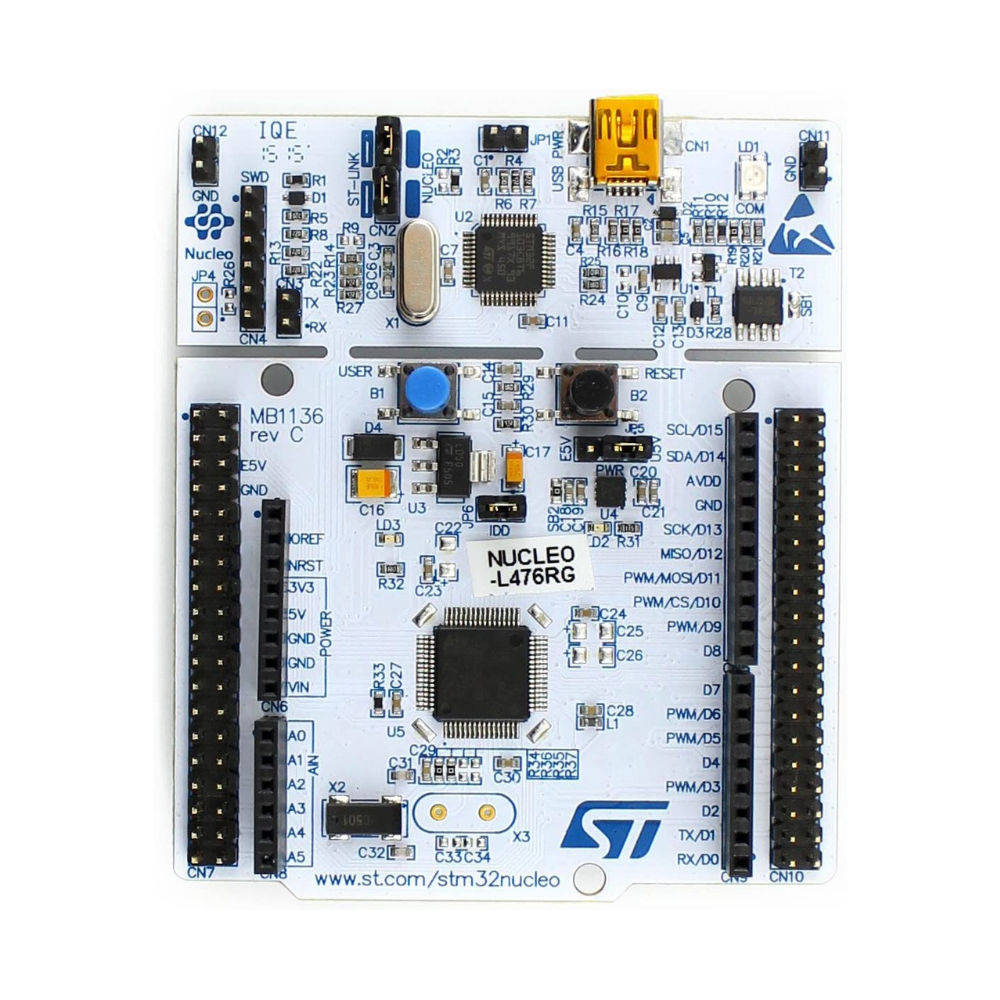
\includegraphics[width=0.5\textwidth]{assets/l476rg.png}
\caption{STM32 NUCLEO-L476RG development board used as the MCU host platform.}
\end{figure}

\begin{figure}[h]
\centering
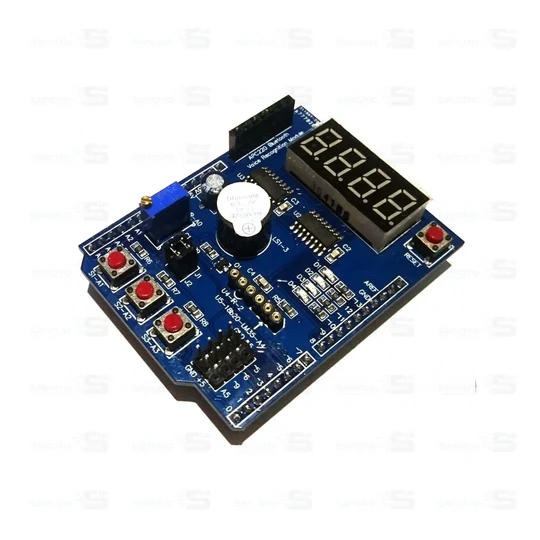
\includegraphics[width=0.36\textwidth]{assets/mfs.png}
\caption{Multi-Function Shield providing the 4-digit display, LEDs, buzzer, and buttons.}
\end{figure}

\begin{figure}[h]
\centering
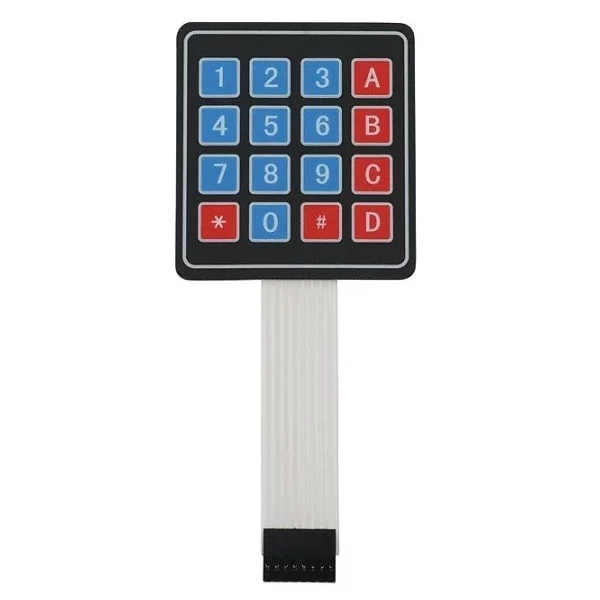
\includegraphics[width=0.34\textwidth]{assets/zrx543.png}
\caption{4x4 matrix keypad used as the primary secure input device.}
\end{figure}

\clearpage

\section{Hardware Architecture}

\subsection{System View}

\begin{tabularx}{\textwidth}{>{\bfseries}l X}
User / Administrator & Operates the front panel, enters user or admin credentials, and receives status feedback. \\
Matrix keypad & Primary secure input surface for digits \texttt{0-9}, control keys \texttt{*} and \texttt{\#}, and function keys \texttt{A-D}. \\
Shield push buttons & Secondary shortcut inputs mapped by firmware to logical keys \texttt{A}, \texttt{\#}, and \texttt{*}. \\
STM32L476RG MCU & Schedules periodic activities, scans inputs, runs the state machine, and drives all outputs. \\
Seven-segment display & Presents messages such as \texttt{SAFE}, \texttt{OPEN}, \texttt{FAIL}, timers, and menu labels. \\
LEDs and buzzer & Provide status indication for armed, admin, success, error, and lockout conditions. \\
\end{tabularx}

\subsection{Control Partitioning}

The design separates logical behavior from hardware-specific I/O:

\begin{itemize}[leftmargin=1.5em]
\item \texttt{src/app\_fsm.c} owns safe behavior, security states, and user/admin workflows
\item \texttt{src/hw.c} owns GPIO configuration, keypad scanning, display multiplexing, LEDs, buzzer, and low-power waiting
\item \texttt{src/display.c}, \texttt{src/indicators.c}, \texttt{src/keypad.c}, and \texttt{src/storage.c} define logical models that decouple the application from register-level code
\end{itemize}

This partitioning is important because the safe logic can be validated independently from the board,
while the board support layer contains the timing-sensitive electrical behavior.

\subsection{Hardware Blocks and Responsibilities}

\begin{longtable}{p{0.25\textwidth} p{0.45\textwidth} p{0.22\textwidth}}
\toprule
\textbf{Block} & \textbf{Role in the system} & \textbf{Firmware boundary} \\
\midrule
\endhead
STM32L476RG & Main controller, scheduler clock source, GPIO host, and low-power execution target & \texttt{src/main.c}, \texttt{src/hw.c} \\
Multi-Function Shield display & 4-digit numeric and text feedback & \texttt{src/display.c} and display drive logic in \texttt{src/hw.c} \\
Shield LEDs & Armed, admin, success, error, and lockout indication & \texttt{src/indicators.c} and LED mapping in \texttt{src/hw.c} \\
Shield buzzer & Audible keypress and alarm feedback & \texttt{src/indicators.c} and buzzer pulse logic in \texttt{src/hw.c} \\
Shield buttons & Shortcut inputs mapped to logical keys \texttt{A}, \texttt{\#}, and \texttt{*} & debounce and key injection logic in \texttt{src/hw.c} \\
4x4 keypad & Primary front-panel input & matrix scan and debounce logic in \texttt{src/hw.c} \\
\bottomrule
\end{longtable}

\subsection{I/O Mapping}

The implementation in \texttt{src/hw.c} defines the active hardware mapping used by the prototype.

\subsubsection*{Shield connections}

\begin{tabularx}{\textwidth}{l l X}
\toprule
\textbf{Function} & \textbf{MCU pin} & \textbf{Notes} \\
\midrule
Shift register latch & \texttt{PB5} & Shield display drive \\
Shift register clock & \texttt{PA8} & Shield display drive \\
Shift register data & \texttt{PA9} & Shield display drive \\
Buzzer & \texttt{PB3} & Active-low behavior selected in \texttt{include/config.h} \\
LED1 & \texttt{PA5} & Error and lockout patterns \\
LED2 & \texttt{PA6} & Armed and admin patterns \\
LED3 & \texttt{PA7} & Admin patterns \\
LED4 & \texttt{PB6} & Success indication \\
Shield button S1 & \texttt{PA1} & Injected as key \texttt{A} \\
Shield button S2 & \texttt{PA4} & Injected as key \texttt{\#} \\
Shield button S3 & \texttt{PB0} & Injected as key \texttt{*} \\
\bottomrule
\end{tabularx}

\subsubsection*{External keypad connections}

\begin{tabularx}{0.6\textwidth}{l l}
\toprule
\textbf{Keypad signal} & \textbf{MCU pin} \\
\midrule
Row 1 & \texttt{PC10} \\
Row 2 & \texttt{PC11} \\
Row 3 & \texttt{PC12} \\
Row 4 & \texttt{PD2} \\
Column 1 & \texttt{PC8} \\
Column 2 & \texttt{PC6} \\
Column 3 & \texttt{PC5} \\
Column 4 & \texttt{PC4} \\
\bottomrule
\end{tabularx}

\subsubsection*{Keypad map}

\begin{verbatim}
1 2 3 A
4 5 6 B
7 8 9 C
* 0 # D
\end{verbatim}

\subsection{Electrical Interaction Model}

The hardware layer performs these low-level tasks:

\begin{itemize}[leftmargin=1.5em]
\item configures GPIO for output, pull-up input, or analog high-impedance mode
\item scans keypad rows against pulled-up columns and accepts exactly one stable pressed key
\item debounces both keypad and shield buttons before generating logical key events
\item multiplexes the four display digits at a fixed refresh cadence
\item converts ASCII characters into seven-segment patterns
\item drives LED patterns according to logical application state
\item pulses the buzzer for keypress, success, error, or periodic lockout feedback
\item sleeps with \texttt{\_\_WFI()} between scheduled activities
\end{itemize}

One notable implementation detail is the buzzer idle strategy: when the buzzer is silent, its pin
is parked in analog mode so the shield sees a high-impedance state instead of a guessed inactive
logic level.

\section{Firmware Architecture}

\subsection{Layered View}

\begin{tabularx}{\textwidth}{>{\bfseries}l X}
\texttt{src/main.c} & Deterministic superloop scheduler and timing orchestration. \\
\texttt{src/hw.c} & Board support layer: GPIO setup, input scan, display refresh, LED drive, buzzer drive, and sleep behavior. \\
\texttt{src/app\_fsm.c} & Application state machine and security policy. \\
\texttt{src/display.c}, \texttt{src/indicators.c}, \texttt{src/keypad.c}, \texttt{src/storage.c} & Logical models and data abstractions consumed by the application and hardware layers. \\
\end{tabularx}

\subsection{Main Execution Model}

The firmware is single-threaded and built around a deterministic superloop. \texttt{main()} performs
three periodic activities using millisecond time derived from SysTick:

\begin{tabularx}{\textwidth}{l l X}
\toprule
\textbf{Activity} & \textbf{Period} & \textbf{Purpose} \\
\midrule
Input scan & \texttt{1 ms} & Poll keypad matrix and shield buttons \\
App tick & \texttt{50 ms} & Process queued key events and advance the state machine \\
Display/output refresh & \texttt{2 ms} & Multiplex display digits and apply LED/buzzer outputs \\
\bottomrule
\end{tabularx}

This timing model keeps acquisition, policy, and output refresh separate:

\begin{itemize}[leftmargin=1.5em]
\item input acquisition stays fast enough for responsive key handling
\item application policy remains coarse-grained and easier to reason about
\item display multiplexing remains independent from business logic timing
\end{itemize}

\subsection{Firmware Data Flow}

\begin{enumerate}[leftmargin=1.7em]
\item \texttt{hw\_poll\_inputs()} scans the physical keypad and push buttons.
\item Stable physical events are translated into logical keys and pushed into the keypad queue.
\item \texttt{app\_tick()} drains the queue and runs the state machine.
\item The state machine updates logical display, indicator, and storage state.
\item \texttt{hw\_apply\_outputs()} reads the logical output intent and drives the display, LEDs, and buzzer.
\end{enumerate}

\subsection{Core Modules}

\subsubsection*{\texttt{src/main.c}}

Provides the scheduler shell:

\begin{itemize}[leftmargin=1.5em]
\item initializes the hardware boundary and application model
\item tracks last execution time for each periodic task
\item runs periodic input polling, application ticking, and output refresh
\item enters low-power wait between events
\end{itemize}

\subsubsection*{\texttt{src/app\_fsm.c}}

Implements the safe's control policy as a finite-state machine. It is the main source of truth for
security behavior and operator interaction.

Main responsibilities:

\begin{itemize}[leftmargin=1.5em]
\item accept logical key events
\item validate user and admin PINs
\item maintain state transitions and timeouts
\item control lockout behavior
\item manage admin menu actions
\item render logical display text and indicator patterns
\end{itemize}

\subsubsection*{\texttt{src/storage.c}}

Stores mutable configuration and counters:

\begin{itemize}[leftmargin=1.5em]
\item user PIN
\item admin PIN
\item lockout duration
\item sound enabled flag
\item maximum failed attempts
\item failed-attempt counter
\end{itemize}

The current storage model is volatile only. A power cycle restores default values. The module shape
intentionally allows a later replacement with non-volatile persistence without changing the application contract.

\subsubsection*{\texttt{src/keypad.c}}

Provides a bounded key event queue. This prevents the state machine from depending directly on scan
timing and gives the application one stable input abstraction.

\subsubsection*{\texttt{src/display.c}}

Maintains a logical four-character display buffer with helpers for fixed text, numeric rendering,
and masked progress feedback during PIN entry.

\subsubsection*{\texttt{src/indicators.c}}

Maintains the logical LED and buzzer intent chosen by the state machine, including enforcement of
the global sound enable flag.

\subsubsection*{\texttt{src/hw.c}}

Translates logical display and indicator intent into physical GPIO behavior and converts physical
input activity into stable logical key events.

\subsection{Application States}

\begin{tabularx}{\textwidth}{l X}
\toprule
\textbf{State} & \textbf{Meaning} \\
\midrule
\texttt{STATE\_IDLE} & Armed and waiting for input \\
\texttt{STATE\_ENTER\_PIN} & User PIN entry in progress \\
\texttt{STATE\_VALIDATE\_PIN} & PIN verification step \\
\texttt{STATE\_ACCESS\_GRANTED} & Transient success state \\
\texttt{STATE\_ACCESS\_DENIED} & Transient failure state \\
\texttt{STATE\_LOCKOUT} & Timed lockout after too many failed attempts \\
\texttt{STATE\_ADMIN\_AUTH} & Admin PIN entry \\
\texttt{STATE\_ADMIN\_MENU} & Administrator menu selection \\
\texttt{STATE\_CHANGE\_PIN} & User PIN update workflow \\
\texttt{STATE\_SET\_LOCKOUT} & Lockout duration configuration workflow \\
\texttt{STATE\_DIAGNOSTICS} & Failure-count and status summary view \\
\bottomrule
\end{tabularx}

\subsection{User and Admin Interaction Model}

\subsubsection*{User path}

\begin{enumerate}[leftmargin=1.7em]
\item The display shows \texttt{SAFE}.
\item The user enters four digits.
\item \texttt{\#} submits the PIN.
\item A valid PIN shows \texttt{OPEN} and success feedback.
\item An invalid PIN shows \texttt{FAIL}.
\item After the configured attempt threshold, the safe enters timed lockout and the display shows the remaining seconds.
\end{enumerate}

\subsubsection*{Admin path}

\begin{enumerate}[leftmargin=1.7em]
\item The operator enters admin mode with \texttt{A}.
\item A 6-digit admin PIN is entered and submitted with \texttt{\#}.
\item On success, the firmware enters \texttt{STATE\_ADMIN\_MENU}.
\item \texttt{B} and \texttt{C} cycle forward and backward through menu items.
\item \texttt{\#} activates the selected function.
\item \texttt{*} returns to idle or backs out of the current admin workflow.
\end{enumerate}

Available admin menu functions:

\begin{itemize}[leftmargin=1.5em]
\item \texttt{PINC}: change the user PIN
\item \texttt{TIME}: set lockout duration in seconds
\item \texttt{BEEP}: enable or disable sound feedback
\item \texttt{FAIL}: show failed-attempt count
\item \texttt{DIAG}: show sound status and lockout time summary
\end{itemize}

\section{Security-Relevant Behavior}

The current implementation already includes several safe-controller protections:

\begin{itemize}[leftmargin=1.5em]
\item fixed-length validation for user and admin PINs
\item bounded keypad queue capacity
\item debounced physical inputs before key acceptance
\item rejection of unsupported keys at the queue boundary
\item automatic failed-attempt tracking
\item timed lockout after the configured threshold
\item explicit separation between normal-user and admin workflows
\end{itemize}

Current prototype limits to be aware of:

\begin{itemize}[leftmargin=1.5em]
\item credentials are stored only in volatile memory
\item there is no tamper sensing, enclosure switch, or secure element
\item PIN comparison is functional rather than hardened against side-channel analysis
\item this is a control-panel prototype, not a certified high-security safe product
\end{itemize}

\section{Relevant Source Map}

\begin{tabularx}{\textwidth}{l X}
\toprule
\textbf{Concern} & \textbf{Path} \\
\midrule
application logic / state machine & \texttt{src/app\_fsm.c}, \texttt{include/app\_fsm.h} \\
hardware boundary & \texttt{src/hw.c}, \texttt{include/hw.h} \\
display model & \texttt{src/display.c}, \texttt{include/display.h} \\
indicator model & \texttt{src/indicators.c}, \texttt{include/indicators.h} \\
keypad queue & \texttt{src/keypad.c}, \texttt{include/keypad.h} \\
configuration and limits & \texttt{include/config.h} \\
mutable settings & \texttt{src/storage.c}, \texttt{include/storage.h} \\
logic tests & \texttt{test/test\_safe\_logic.c} \\
\bottomrule
\end{tabularx}

\section{Summary}

This repository implements a compact but well-partitioned embedded safe controller:

\begin{itemize}[leftmargin=1.5em]
\item hardware-specific code is isolated in the board support layer
\item security and operator behavior are concentrated in a finite-state machine
\item logical models decouple policy from display and GPIO details
\item the prototype is suitable for demonstration, validation, and later extension toward persistent storage or actuator integration
\end{itemize}

The Markdown file remains the easiest version-controlled source for review, while this PDF companion
is better suited for submission, sharing, and printing.

\end{document}
